\documentclass{article}
\usepackage[letterpaper, text={6.875in,8.875in}, top=1in]{geometry}
\usepackage{times}     % Times text font, as in the sample
\usepackage{booktabs}  % \toprule / \midrule / \bottomrule tables
\usepackage{titlesec}
\usepackage{amssymb}
\usepackage[ruled,vlined,linesnumbered]{algorithm2e}
\usepackage{amsmath}
\usepackage{hyperref}
\usepackage{natbib}
\usepackage{accents}
\usepackage{graphicx}
\usepackage{subcaption}
\usepackage{hyperref}
\usepackage[dvipsnames]{xcolor}
\usepackage{parskip}  % blank line in the source = visible gap between paragraphs, no indent
\captionsetup{font=small, labelsep=period}  % "Table 1." / "Figure 1." small captions
\renewcommand{\thempfootnote}{\arabic{mpfootnote}}

\definecolor{urlBlue}{rgb}{0.21,0.49,0.74}
\hypersetup{
    colorlinks=true,
    linkcolor=urlBlue,    % Color of internal links (sections, pages)
    urlcolor=urlBlue,     % Color of URL links (web addresses)
    citecolor=urlBlue     % Color of citation links
}

\DeclareMathOperator*{\argmax}{arg\,max}
\DeclareMathOperator*{\argmin}{arg\,min}
\DeclareMathOperator*{\sol}{\text{sol}}

\newcommand{\ubar}[1]{\underaccent{\bar}{#1}}
\newcommand{\norm}[2]{\left\lVert#1\right\rVert\right_{#2}}

\setlength{\parindent}{0pt}
\raggedbottom  % don't stretch paragraph gaps to fill each column
\pagestyle{empty}  % no page numbers

% Section headings like the sample: large bold, flush left
\titleformat*{\section}{\large\bfseries}
\titlespacing*{\section}{0pt}{12pt plus 3pt minus 2pt}{6pt}

\graphicspath{{figures/}}

\newcommand{\question}[1]{\par\medskip\noindent\textit{#1}\par\smallskip}

\begin{document}
\begin{center}
{\Large\bfseries ORIE 5380 Course Project Report: Part 1 \par}
\vspace{1.2em}
{\normalsize David Johnson (dmj68), Priyansh Raval (pr496) \par}
\vspace{2em}
\end{center}

\textbf{Use of AI.} 
We formulated the models ourselves on a whiteboard, then used Anthropic's Claude and OpenAI's ChatGPT to write up those formulations.

%--------------------------------------------------------------------
\section*{Question 1: Minimize Mean Travel Time}

Select $p$ of $N$ stores to minimize the average travel time of $M$ customers.
Let $t_{ij}$ be the travel time from customer $i$ to store $j$.

\subsection*{Decision Variables}
\[
y_j = \begin{cases}
1 & \text{if store $j$ is selected},\\
0 & \text{otherwise},
\end{cases}
\qquad
x_{ij} = \begin{cases}
1 & \text{if customer $i$ is assigned to store $j$},\\
0 & \text{otherwise}.
\end{cases}
\]
Both variables are binary, for all $i\in[M]$ and $j\in[N]$.

\subsection*{Objective Function}
\begin{equation}
\min_{y,x}\quad \frac{1}{M}\sum_{i=1}^{M}\sum_{j=1}^{N}t_{ij}x_{ij}.
\label{eq:mean-obj}
\end{equation}
This minimizes the mean travel time to customers' assigned stores. Each customer is
assigned to a nearest selected store in an optimal solution.

\subsection*{Constraints}
\begin{center}
\begin{tabular}{@{}p{0.49\textwidth}p{0.47\textwidth}@{}}
\toprule
\textbf{Constraint} & \textbf{What it enforces} \\
\midrule
$\sum_{j=1}^{N}y_j=p$ & Select exactly $p$ stores. \\[6pt]
$\sum_{j=1}^{N}x_{ij}=1\quad \forall i\in[M]$ & Assign each customer to exactly one store. \\[6pt]
$x_{ij}\le y_j\quad \forall i\in[M],\ j\in[N]$ & Allow assignments only to selected stores. \\[6pt]
$y_j\in\{0,1\}\quad \forall j\in[N]$ & Make store selection binary. \\[6pt]
$x_{ij}\in\{0,1\}\quad \forall i\in[M],\ j\in[N]$ & Make customer assignments binary. \\
\bottomrule
\end{tabular}
\end{center}

%--------------------------------------------------------------------
\section*{Question 2: Minimize Worst-Case Travel Time}

Select $p$ stores to minimize the maximum customer travel time, using the same $t_{ij}$.

\subsection*{Decision Variables}
Use the binary variables $y_j$ and $x_{ij}$ from Question 1. Add a continuous variable
$T\ge0$ bounding every customer's assigned travel time.

\subsection*{Objective Function}
\begin{equation}
\min_{y,x,T}\quad T.
\label{eq:max-obj}
\end{equation}
This minimizes the worst-case customer travel time.

\subsection*{Constraints}
\begin{center}
\begin{tabular}{@{}p{0.49\textwidth}p{0.47\textwidth}@{}}
\toprule
\textbf{Constraint} & \textbf{What it enforces} \\
\midrule
$\sum_{j=1}^{N}t_{ij}x_{ij}\le T\quad \forall i\in[M]$ & Bound every customer's travel time by $T$. \\[6pt]
$\sum_{j=1}^{N}y_j=p$ & Select exactly $p$ stores. \\[6pt]
$\sum_{j=1}^{N}x_{ij}=1\quad \forall i\in[M]$ & Assign each customer to exactly one store. \\[6pt]
$x_{ij}\le y_j\quad \forall i\in[M],\ j\in[N]$ & Allow assignments only to selected stores. \\[6pt]
$y_j\in\{0,1\}\quad \forall j\in[N]$ & Make store selection binary. \\[6pt]
$x_{ij}\in\{0,1\}\quad \forall i\in[M],\ j\in[N]$ & Make customer assignments binary. \\
$T\ge0$ & Keep the travel-time bound nonnegative. \\
\bottomrule
\end{tabular}
\end{center}

Customers need not be assigned to their nearest selected store if their travel time
remains at most $T$. Reassigning them to their nearest selected store cannot increase
$T$ and gives the nearest-store travel times requested for reporting.

%--------------------------------------------------------------------
\section*{Question 3: Optimization performance}
\question{Implement both models using \texttt{gurobipy}, test each for $p = 1, \ldots, 10$ with a one-minute time limit, and plot runtime and optimality gap versus $p$. Which model performed better in terms of runtime? Do you think the difference in optimization performance would be an important consideration in practice?}

The existing notebook results use continuous assignment variables $x_{ij}\in[0,1]$, rather than the binary assignments formulated above. The continuous formulations have the same optimal objective values, but their runtimes do not measure the binary formulations. These runs used Gurobi~14.0 with a 60-second time limit (\texttt{TimeLimit = 60}). Figure~\ref{fig:runtime-gap} shows runtime and optimality gap versus $p$, and Table~\ref{tab:runtime} lists the runtimes.

\begin{figure}[htbp]
    \centering
    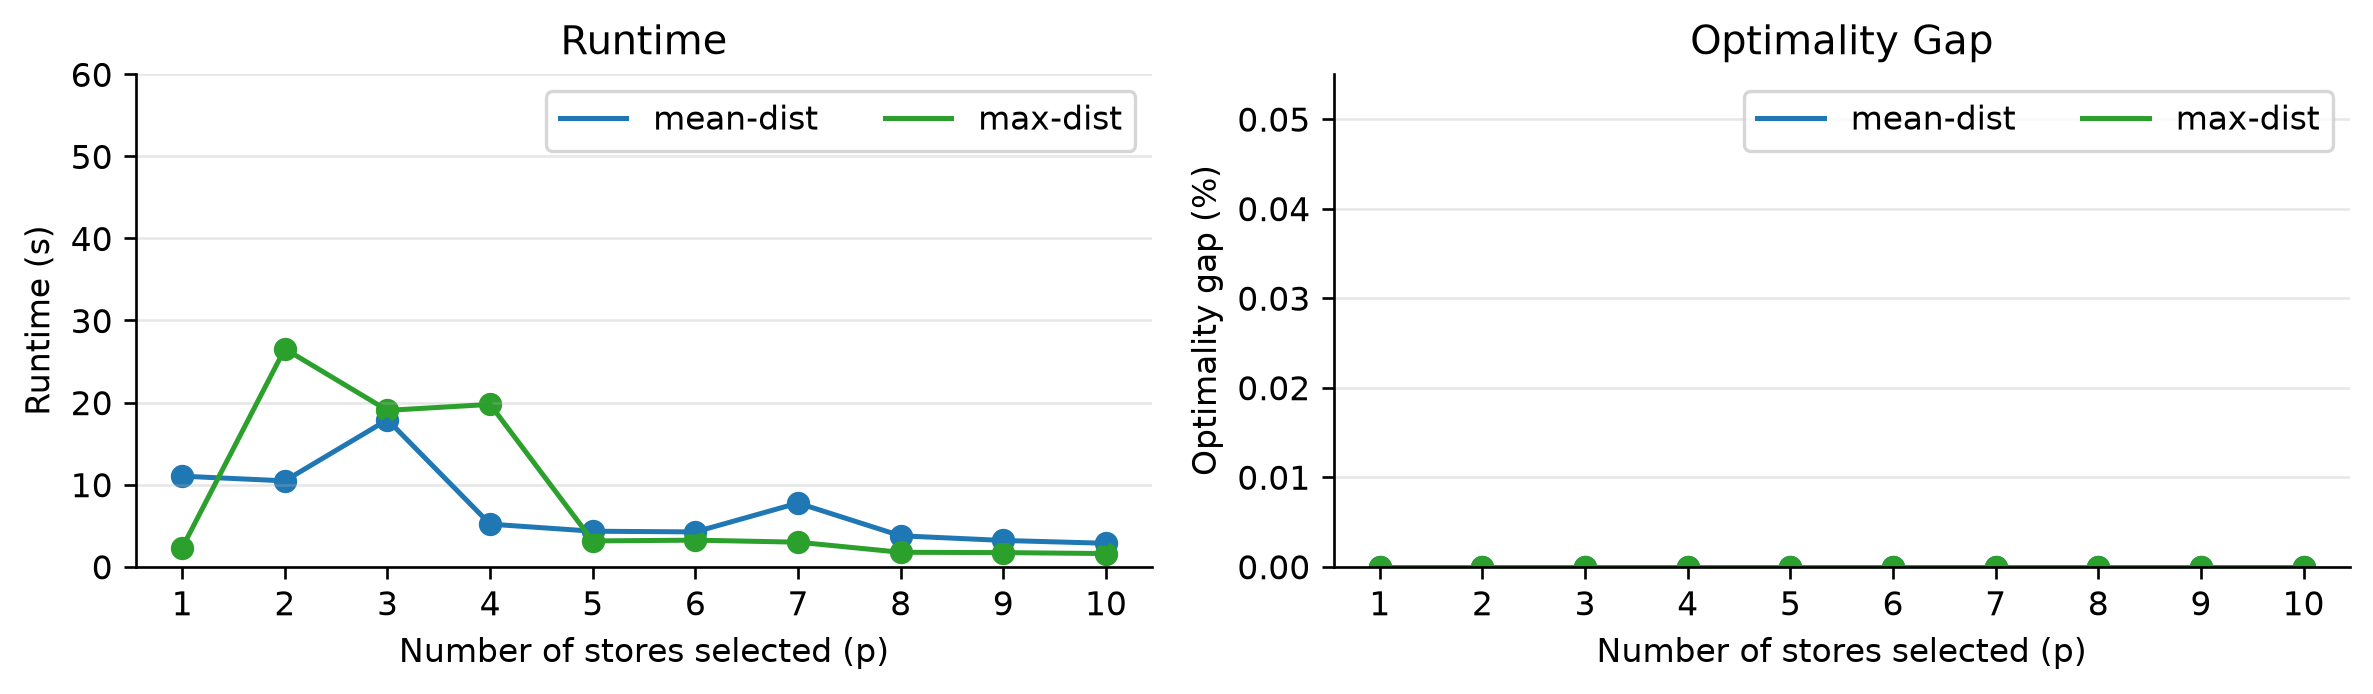
\includegraphics[width=\textwidth]{part1_runtime_gap.png}
    \caption{Gurobi runtime (left) and final optimality gap (right) versus the number of selected stores $p$ for the mean-dist (blue) and max-dist (green) models.}
    \label{fig:runtime-gap}
\end{figure}

\begin{table}[htbp]
\centering
\small
\begin{tabular}{l*{10}{c}c}
\toprule
$p$ & 1 & 2 & 3 & 4 & 5 & 6 & 7 & 8 & 9 & 10 & Total \\ \midrule
mean-dist runtime (s) & 0.35 & 4.80 & 4.01 & 2.80 & 2.36 & 2.19 & 2.80 & 1.95 & 1.76 & 1.68 & 24.71 \\
max-dist runtime (s)  & 0.44 & 17.53 & 49.66 & 22.39 & 6.67 & 9.58 & 3.93 & 3.70 & 3.18 & 1.43 & 118.52 \\ \bottomrule
\end{tabular}
\caption{Runtime for each model and value of $p$. Every run terminated with a proven optimal solution (0\% optimality gap).}
\label{tab:runtime}
\end{table}

%--------------------------------------------------------------------
\section*{Question 4: Average and worst-case travel time versus $p$}
\question{Create a plot showing the average and worst-case travel time for each model and value of $p$. Describe how the average and worst-case customer travel time change as you include more locations in the pilot.}

\begin{figure}[htbp]
    \centering
    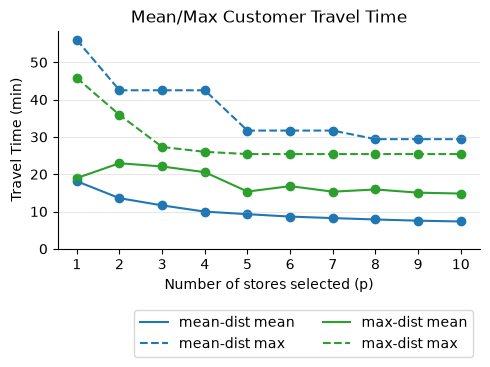
\includegraphics[width=0.6\textwidth]{part1_mean_max_time.png}
    \caption{Mean (solid) and maximum (dashed) customer travel time versus $p$ for the mean-dist (blue) and max-dist (green) models. For mean-dist, travel times are measured to each customer's closest selected store. For max-dist, each customer's travel time is the trip-weighted average $\sum_j t_{ij} x_{ij}$ from the model's solution.}
    \label{fig:mean-max}
\end{figure}

%--------------------------------------------------------------------
\section*{Question 5: Spatial comparison for $p = 5$}
\question{Spatially visualize the closest store for each customer and minimum travel time for each customer for both models, including the closest store figure for $p = 5$ for both models. Which model do you think results in a better solution? Justify your answer.}

%--------------------------------------------------------------------
\section*{Question 6: Travel distance instead of travel time}
\question{A colleague suggests using travel distances instead of OSRM traffic-free travel times. Could travel distances easily be incorporated into the model? Do you think using travel distance instead of travel time is an improvement to the model?}

\end{document}
